\documentclass[border=4pt]{standalone}
\usepackage[T1]{fontenc}
\usepackage{times}
\usepackage{tikz}
\usepackage{amsmath}
\usepackage{amssymb}
\usetikzlibrary{arrows.meta,positioning,backgrounds,fit,calc,shapes.geometric}
\DeclareMathSizes{8}{10}{7}{5}

% ---- palette (unchanged from fig1_paper_overview.tex) ----
\definecolor{stagefill}{HTML}{F4F6FB}
\definecolor{stageline}{HTML}{C7CFE0}
\definecolor{ink}{HTML}{1F2733}
\definecolor{flow}{HTML}{5B6B86}
\definecolor{rootc}{HTML}{2B2F3A}
\definecolor{bannerfill}{HTML}{EAEEF7}
\definecolor{bannerline}{HTML}{B7C2D8}
\definecolor{estc}{HTML}{3F7CAC}
\definecolor{truthc}{HTML}{2B2F3A}
\definecolor{nullc}{HTML}{B9C0CE}
\definecolor{okc}{HTML}{4FA06B}

\begin{document}
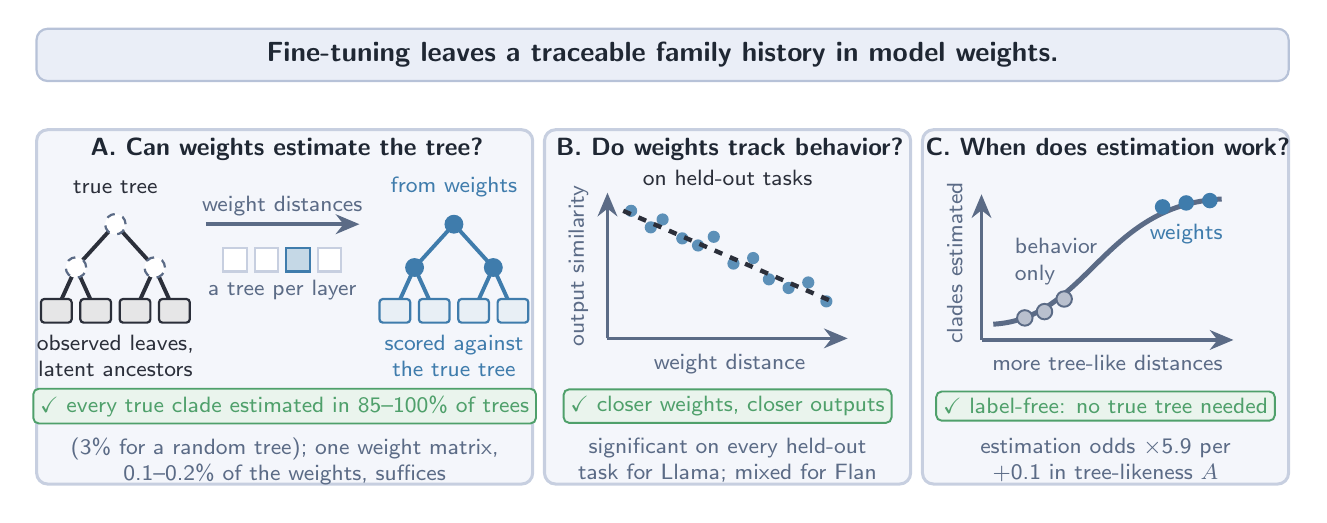
\begin{tikzpicture}[
  font=\sffamily,
  >={Stealth[length=3.0mm,width=2.5mm]},
  panel/.style={draw=stageline,line width=1.1pt,rounded corners=4pt,fill=stagefill},
  ptitle/.style={font=\sffamily\small\bfseries,text=ink},
  lab/.style={font=\sffamily\footnotesize},
  scap/.style={font=\sffamily\footnotesize,text=flow,align=center},
  mdl/.style={draw=truthc,fill=white,rounded corners=1.2pt,minimum width=3.9mm,minimum height=3.0mm,line width=0.8pt,inner sep=0pt},
  latent/.style={circle,draw=flow,dashed,fill=white,line width=0.8pt,inner sep=0pt,minimum size=2.6mm},
  layer/.style={draw=stageline,fill=white,line width=0.8pt,minimum width=3.0mm,minimum height=3.0mm,inner sep=0pt},
]

% ===================== TOP CLAIM BANNER =====================
\node[draw=bannerline,fill=bannerfill,rounded corners=4pt,line width=0.8pt,
      text width=15.55cm,align=center,inner sep=5pt,
      font=\sffamily\normalsize\bfseries,text=ink] (banner) at (8.05,5.40)
  {Fine-tuning leaves a traceable family history in model weights.};

% ===================== PANEL A: primary contribution =====================
\begin{scope}
  \node[panel,minimum width=6.3cm,minimum height=4.5cm] (PA) at (3.25,2.2){};
  \node[ptitle,anchor=north] at (PA.north) {\,A.\ Can weights estimate the tree?};

  % true tree: only the leaves are observed; ancestors are latent
  \node[lab,text=truthc] at (1.10,3.72) {true tree};
  \coordinate (tr) at (1.10,3.25);
  \coordinate (ta) at (0.60,2.70); \coordinate (tb) at (1.60,2.70);
  \coordinate (ta1) at (0.35,2.15);\coordinate (ta2) at (0.85,2.15);
  \coordinate (tb1) at (1.35,2.15);\coordinate (tb2) at (1.85,2.15);
  \draw[truthc,line width=1.4pt] (tr)--(ta) (tr)--(tb) (ta)--(ta1) (ta)--(ta2) (tb)--(tb1) (tb)--(tb2);
  \foreach \p in {tr,ta,tb}{\node[latent] at (\p){};}
  \foreach \p in {ta1,ta2,tb1,tb2}{\node[mdl,fill=truthc!12] at (\p){};}
  \node[scap,text=truthc] at (1.10,1.58) {observed leaves,\\latent ancestors};

  % middle: each weight layer is a gene with its own tree
  \draw[->,line width=1.4pt,draw=flow] (2.25,3.25)--(4.20,3.25);
  \node[lab,text=flow] at (3.22,3.48) {weight distances};
  \foreach \x in {2.62,3.02,3.42,3.82}{\node[layer] at (\x,2.80){};}
  \node[layer,draw=estc,fill=estc!30] at (3.42,2.80){};
  \node[lab,text=flow] at (3.22,2.42) {a tree per layer};

  % estimated tree
  \node[lab,text=estc] at (5.40,3.72) {from weights};
  \coordinate (er) at (5.40,3.25);
  \coordinate (ea) at (4.90,2.70); \coordinate (eb) at (5.90,2.70);
  \coordinate (ea1) at (4.65,2.15);\coordinate (ea2) at (5.15,2.15);
  \coordinate (eb1) at (5.65,2.15);\coordinate (eb2) at (6.15,2.15);
  \draw[estc,line width=1.4pt] (er)--(ea) (er)--(eb) (ea)--(ea1) (ea)--(ea2) (eb)--(eb1) (eb)--(eb2);
  \foreach \p in {er,ea,eb}{\node[circle,fill=estc,inner sep=0pt,minimum size=2.4mm] at (\p){};}
  \foreach \p in {ea1,ea2,eb1,eb2}{\node[mdl,draw=estc,fill=estc!12] at (\p){};}

  \node[scap,text=estc] at (5.40,1.58) {scored against\\the true tree};

  % headline result
  \node[draw=okc,rounded corners=2pt,line width=0.7pt,fill=okc!12,
        font=\sffamily\footnotesize,text=okc,inner sep=2.5pt] at (3.25,0.94)
        {$\checkmark$ every true clade estimated in 85--100\% of trees};
  \node[scap,anchor=north] at (3.25,0.66)
        {(3\% for a random tree); one weight matrix,\\0.1--0.2\% of the weights, suffices};
\end{scope}

% ===================== PANEL B: weights -> held-out behavior =====================
\begin{scope}
  \node[panel,minimum width=4.65cm,minimum height=4.5cm] (PB) at (8.875,2.2){};
  \node[ptitle,anchor=north] at (PB.north) {\,B.\ Do weights track behavior?};
  \node[lab,text=truthc] at (8.875,3.84) {on held-out tasks};

  \begin{scope}[shift={(7.35,1.80)}]
    \draw[->,line width=1.2pt,draw=flow] (0,0)--(3.05,0);
    \draw[->,line width=1.2pt,draw=flow] (0,0)--(0,1.85);
    \node[lab,text=flow,anchor=north] at (1.55,-0.07) {weight distance};
    \node[lab,text=flow,rotate=90,anchor=south] at (-0.12,0.92) {output similarity};
    \foreach \x/\y in {0.30/1.62,0.55/1.41,0.70/1.51,0.95/1.27,1.15/1.18,1.35/1.29,1.60/0.95,1.85/1.02,2.05/0.75,2.30/0.64,2.55/0.71,2.78/0.47}{
      \fill[estc!85!white] (\x,\y) circle (2.2pt);
    }
    \draw[truthc,line width=1.6pt,dashed] (0.20,1.62)--(2.85,0.47);
  \end{scope}
  \node[draw=okc,rounded corners=2pt,line width=0.7pt,fill=okc!12,
        font=\sffamily\footnotesize,text=okc,inner sep=2.5pt] at (8.875,0.94)
        {$\checkmark$ closer weights, closer outputs};
  \node[scap,anchor=north] at (8.875,0.66) {significant on every held-out\\task for Llama; mixed for Flan};
\end{scope}

% ===================== PANEL C: label-free additivity; weights vs behavior =====================
\begin{scope}
  \node[panel,minimum width=4.65cm,minimum height=4.5cm] (PC) at (13.675,2.2){};
  \node[ptitle,anchor=north] at (PC.north) {\,C.\ When does estimation work?};

  \begin{scope}[shift={(12.10,1.78)}]
    \draw[->,line width=1.2pt,draw=flow] (0,0)--(3.20,0);
    \draw[->,line width=1.2pt,draw=flow] (0,0)--(0,1.85);
    \node[lab,text=flow,anchor=north] at (1.60,-0.07) {more tree-like distances};
    \node[lab,text=flow,rotate=90,anchor=south] at (-0.12,0.98) {clades estimated};
    % nonlinear (logistic) association, as in the fractional-logit curve of Fig. 4B
    \draw[flow,line width=1.8pt] (0.15,0.20) .. controls (1.35,0.27) and (1.55,1.72) .. (3.05,1.79);
    % behavior-only (PhyloLM) distances: less tree-like, fewer branches
    \foreach \x/\y in {0.55/0.28,0.80/0.36,1.05/0.52}{
      \fill[nullc] (\x,\y) circle (2.8pt); \draw[flow,line width=0.7pt] (\x,\y) circle (2.8pt);}
    % weight distances: more tree-like, nearly all branches
    \foreach \x/\y in {2.30/1.69,2.60/1.74,2.90/1.77}{\fill[estc] (\x,\y) circle (2.8pt);}
    \node[lab,text=flow,align=left,anchor=south west] at (0.30,0.58) {behavior\\only};
    \node[lab,text=estc,anchor=north] at (2.60,1.60) {weights};
  \end{scope}
  \node[draw=okc,rounded corners=2pt,line width=0.7pt,fill=okc!12,
        font=\sffamily\footnotesize,text=okc,inner sep=2.5pt] at (13.675,0.94)
        {$\checkmark$ label-free: no true tree needed};
  \node[scap,anchor=north] at (13.675,0.66) {estimation odds $\times$5.9 per\\+0.1 in tree-likeness $A$};
\end{scope}

\end{tikzpicture}
\end{document}
